\documentclass[10pt,a4paper]{article}
\usepackage[margin=18mm,top=19mm,bottom=19mm]{geometry}
\usepackage[T1]{fontenc}
\usepackage[utf8]{inputenc}
\usepackage{lmodern,amsmath,amssymb,booktabs,array,graphicx,xcolor,hyperref,float,longtable}
\hypersetup{colorlinks=true,linkcolor=blue!50!black,urlcolor=blue!60!black}
\definecolor{navy}{RGB}{21,46,80}
\definecolor{pale}{RGB}{230,239,248}
\setlength{\parskip}{4pt}\setlength{\parindent}{0pt}\emergencystretch=3em
\newcommand{\sectionline}[1]{\par\vspace{6pt}\noindent{\large\bfseries\color{navy}#1}\par\vspace{3pt}\hrule\vspace{4pt}}
\begin{document}
{\small\color{navy}\bfseries SST-WORKBENCH / A063 / INDEPENDENT NUMERICAL FALSIFIER}\hfill{\footnotesize 13 October 2026}
\vspace{3pt}\hrule\vspace{7pt}
{\LARGE\bfseries Does the Hicks $T(3,4)$ vortex line support a finite stable vortex tube?}\par
{\large A063 v0.2.0 --- analytical/numerical reference report}\par\vspace{5pt}
\fcolorbox{navy}{pale}{\parbox{.965\linewidth}{\textbf{Outcome:} The closed $T(3,4)$ vortex-field-line is independently classified numerically. The tested constant-radius knotted tubular surface is \textbf{not material}, and neighboring winding shows nonzero shear. The existence and nonlinear stability of a differently shaped finite tube remains \textbf{UNRESOLVED}. \par\smallskip\textbf{7 PASS / 2 FAIL / 3 UNRESOLVED}}}
\sectionline{1. Model and falsifiable distinctions}
Inside the spherical Hicks aggregate ($r<a$), the exact axisymmetric streamfunction is
\begin{equation}
\psi=A\!\left[J(\lambda r/a)-(r/a)^2J(\lambda)\right]\!\sin^2\theta,
\quad J(y)=\frac{\sin y}{y}-\cos y.
\end{equation}
With $(s,\phi,z)$, $u_s=-\partial_z\psi/s$, $u_z=\partial_s\psi/s$, $u_\phi=(\lambda/a)\psi/s$; the first root of $\tan\lambda=\lambda$ is $\lambda_1\simeq 4.4934094579$. In this Beltrami branch, $\boldsymbol\omega=(\lambda/a)\mathbf u$, hence a streamline is also a \emph{vorticity line}.

Separate four propositions: (I) a closed knotted line; (II) an embedded geometric neighborhood; (III) an actual vortex-aligned/material surface $\boldsymbol\omega\cdot\mathbf n=0$; (IV) nonlinear time-dependent Euler stability. (I) never implies (III) or (IV).
\sectionline{2. Reproduced orbit and independent topology test}
A new high-accuracy integration gives $s_0/a=\mathbf{0.968309830174}$, winding $W=\mathbf{0.75000000000010}$ and closed-orbit residual $\|X(T)-X(0)\|/a=\mathbf{8.7311e-10}$ over four poloidal turns.

The 3-D polygon was projected along four distinct generic directions (raw crossing counts: 11 / 9 / 13 / 15). For each projection, over/under crossing order yields a Wirtinger/Fox Alexander matrix, and its minor gives the same normalized polynomial:
\begin{equation}
\Delta_{\mathrm{numerical}}(t)=t^6-t^5+t^3-t+1
=\Delta_{T(3,4)}(t),\qquad |\Delta(-1)|=3.
\end{equation}
This is independent of a mere winding-label assignment. Matching the Alexander polynomial is not a unique-knot theorem in isolation; the numerically embedded invariant torus and $(3,4)$ winding supply additional classification evidence.
\begin{figure}[H]\centering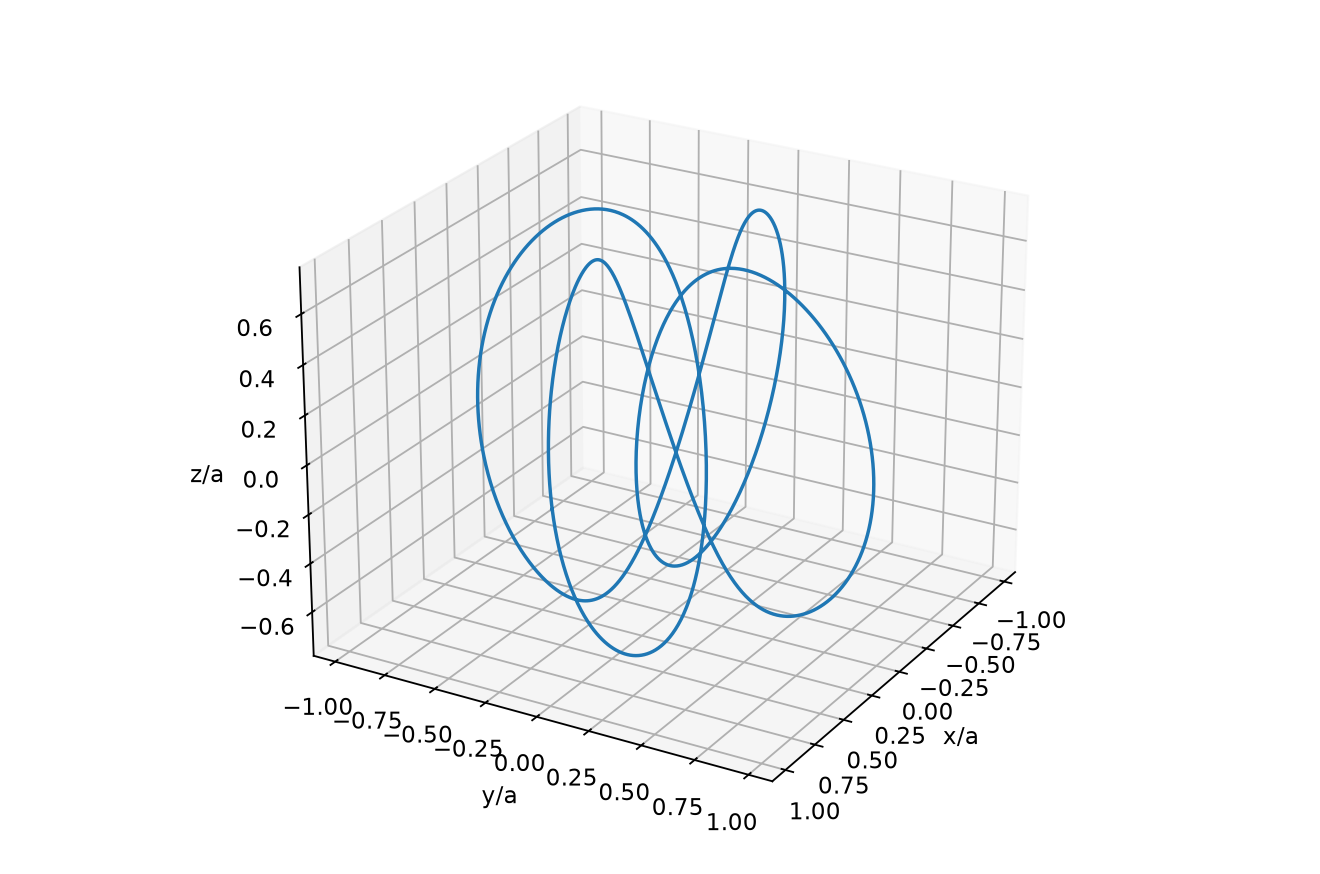
\includegraphics[width=.76\linewidth]{T34_vortex_line.png}\caption{Numerical $T(3,4)$ Hicks-Beltrami vortex line in dimensionless Cartesian coordinates.}\end{figure}
\sectionline{3. Geometric thickening versus material vortex tube}
The sampled minimum curvature-radius proxy is $R_\kappa/a\simeq 0.41864$ and the excluded-neighbor point-distance proxy is $d_{\mathrm{nonlocal}}/a\simeq 0.20135$. The orbit stays at least $0.031690a$ inside the spherical separatrix. These are \textbf{not continuum tube reach bounds} and cannot certify absence of every self-intersection for an arbitrary surface.

For the explicit normal tube $X_{\delta}(\sigma,\vartheta)=X(\sigma)+\delta[\mathbf N(\sigma)\cos\vartheta+\mathbf B(\sigma)\sin\vartheta]$, a material steady tube must satisfy $\mathbf u\cdot\mathbf n=0$ pointwise; and the Beltrami vortex flux satisfies $\boldsymbol\omega\cdot\mathbf n=(\lambda/a)\mathbf u\cdot\mathbf n$. We sampled the actual velocity using the exact field (90 longitudinal points, 16 angular samples, plus a finer 180$\times$24 check).
\begin{table}[H]\centering\begin{tabular}{rrr}\toprule $\delta/a$ & RMS $|u_n|/u_{\rm rms}$ & max $|u_n|/u_{\rm rms}$ \\ \midrule
0.0020 & 0.0024601 & 0.0039760 \\
0.0040 & 0.0049202 & 0.0079704 \\
0.0080 & 0.0098400 & 0.0160367 \\
\bottomrule\end{tabular}\caption{Pointwise normal-velocity diagnostic for an initially constant-radius knot tube.}\end{table}
The zero-radius tangent control is 3.854e-17. The normal leakage is substantially above the preregistered $10^{-4}$ threshold; therefore \textbf{this steady constant-radius normal tube fails the material-surface gate (T5)}. This does not rule out a nonconstant-radius or advected time-dependent tube.
\begin{figure}[H]\centering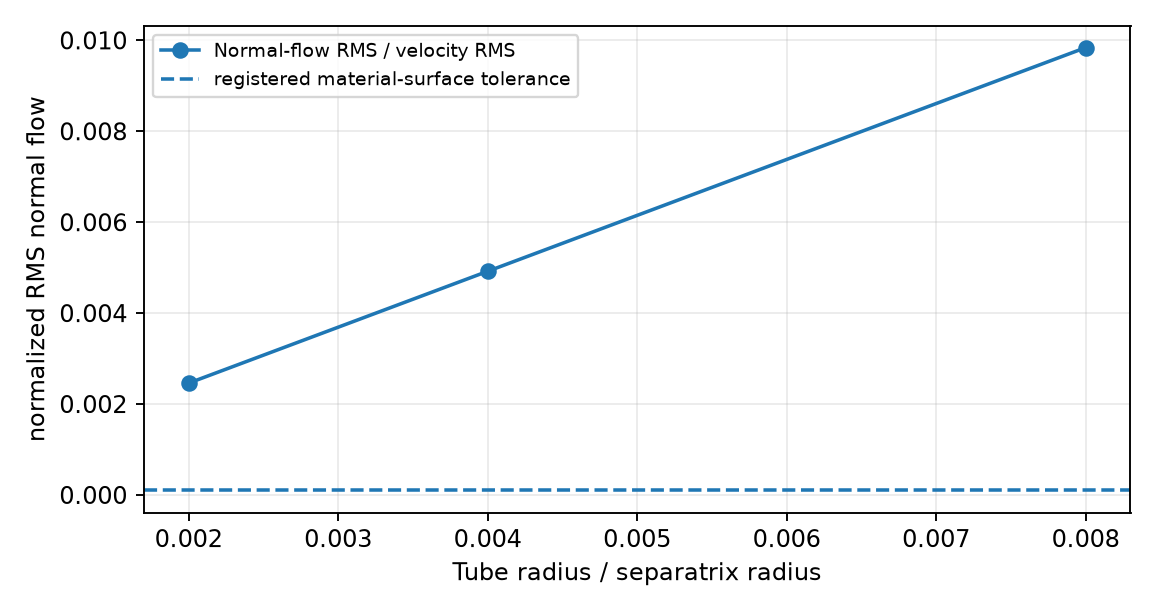
\includegraphics[width=.70\linewidth]{tube_flux.png}\caption{Measured positive normal flow increases with tube radius.}\end{figure}
\sectionline{4. Nearby field lines and pitch-shear test}
The Poincar\'e return rotation $W(s_0)$ has derivative $dW/d(s_0/a)\simeq -0.746819$. Thus a nonzero radial displacement develops azimuthal phase slip after four poloidal circuits:
\begin{equation}\Delta\phi_4\simeq 8\pi\,[W(s_0+\delta s)-3/4].\end{equation}
Therefore a positive-width annulus of neighboring lines does not share the exact same $3{:}4$ closure under this integrable Hicks flow. \textbf{T6 FAIL is a field-line-coherence result, not a time-dependent Euler instability eigenvalue.}
\begin{figure}[H]\centering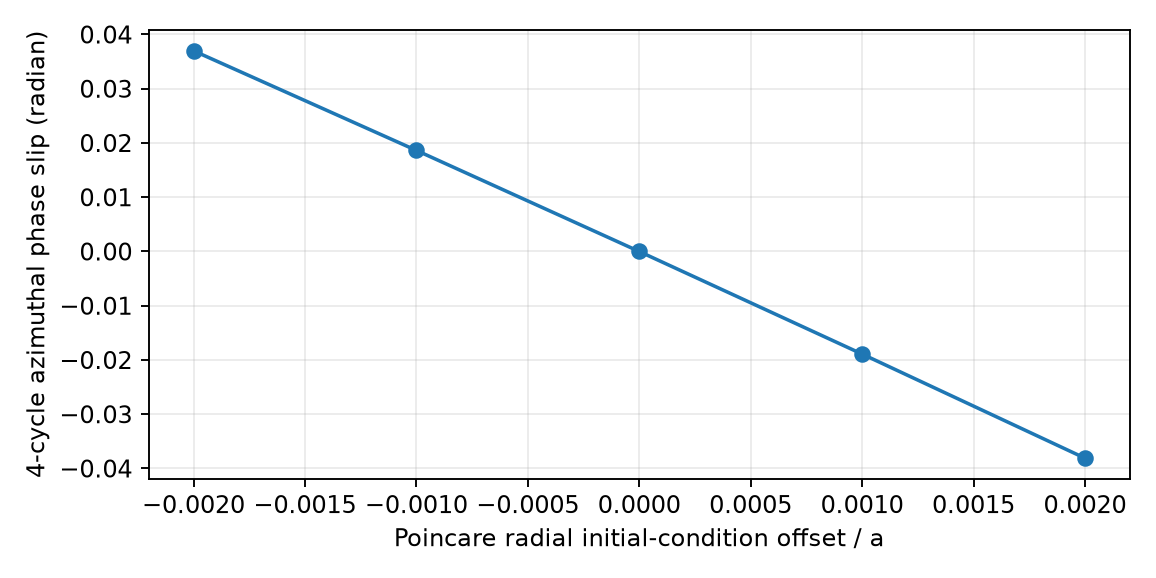
\includegraphics[width=.70\linewidth]{pitch_shear.png}\caption{Neighboring initial conditions produce opposite signed four-period slip.}\end{figure}
\sectionline{5. Finite-time material advection in the prescribed Hicks field}
A material knotted surface (initial $\delta/a=0.004$, 384 markers; confirmation with 720 markers) was transported with $\dot{X}=u_{\rm Hicks}(X)$ while the steady Euler field itself remained fixed. The surface's RMS distance to the original closed knot after four core periods rose to 12.729 times its initial radius (confirmation sample: 12.955 times); intermediate records are stored in the JSON output. This is finite-time kinematic deformation, not a coupled perturbed 3-D Euler evolution.
\begin{figure}[H]\centering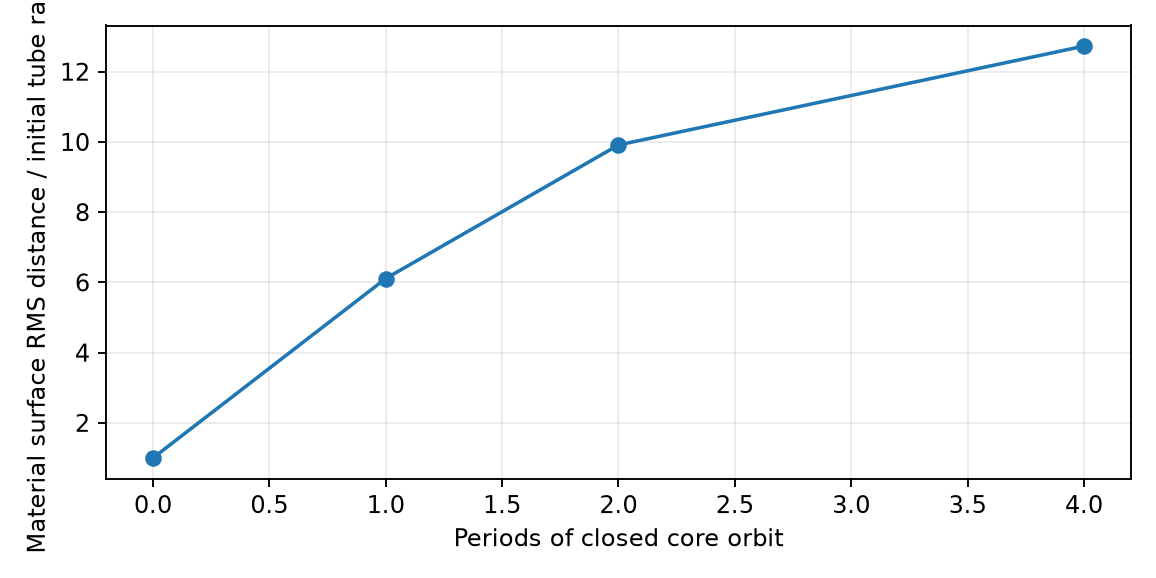
\includegraphics[width=.67\linewidth]{material_advection.png}\caption{Localization of the advected material surface relative to the closed reference knot.}\end{figure}
\sectionline{6. Gate ledger and continuation policy}
\small\begin{longtable}{@{}p{0.075\linewidth}p{0.155\linewidth}>{\raggedright\arraybackslash}p{0.665\linewidth}@{}}\toprule Gate & Result & Qualification question \\ \midrule
\texttt{T0} & \textcolor{green!40!black}{PASS} & Release source/protocol hashes recorded \\
\texttt{T1} & \textcolor{green!40!black}{PASS} & Reproduce a closed rational 3:4 Hicks vortex line \\
\texttt{T2} & \textcolor{green!40!black}{PASS} & Independent Alexander polynomial across generic projection directions \\
\texttt{T3} & \textcolor{green!40!black}{PASS} & Sampled geometric regularity and confinement of a finite normal tube \\
\texttt{T4} & \textcolor{green!40!black}{PASS} & The core is a vortex line: omega=(lambda/a)u \\
\texttt{T5} & \textcolor{red!75!black}{FAIL} & Is a constant-radius knotted tube an instantaneously material/vorticity-aligned surface? \\
\texttt{T6} & \textcolor{red!75!black}{FAIL} & Do adjacent vortex lines have the same 3:4 return rotation (no pitch shear)? \\
\texttt{T7} & \textcolor{green!40!black}{PASS} & Distributed full-sphere vorticity control (not a compact isolated knot tube) \\
\texttt{T8A} & \textcolor{green!40!black}{PASS} & Prescribed-field material advection deformation documented \\
\texttt{T8} & \textcolor{orange!75!black}{UNRESOLVED} & True finite-core stability under 3D perturbed Euler evolution \\
\texttt{T9} & \textcolor{orange!75!black}{UNRESOLVED} & Independent C++ FP64 and canonical v1.0.7 FREEZE/CERTIFY \\
\texttt{T10} & \textcolor{orange!75!black}{UNRESOLVED} & Can any finite topologically consistent dynamically stable vortex tube be constructed? \\
\bottomrule\end{longtable}\normalsize
A scientific FAIL never stops later diagnostic gates. T8A PASS certifies execution of the prescribed-field deformation measurement, not stability. Gates T8 and T9 remain open, rather than being relabeled PASS: no three-dimensional, pressure-coupled perturbed Euler evolution or independent native C++ FP64/canonical-framework certification has been performed.
\sectionline{7. What a decisive follow-up must demonstrate}
Pre-register: a finite smooth tubular surface with independent knot invariant and positive clearance; a flux condition $\boldsymbol\omega\cdot\mathbf n=0$ (or an explicitly time-dependent material-boundary evolution law); constrained-energy stationarity; reproducible linearized-Euler spectra; three spatial resolutions, at least three perturbation amplitudes, and non-linear bounded deformation for 10 core periods, with energy/helicity, divergence, topology and pressure-Poisson audits. Source-independent carriers must be identified separately (E013), not silently substituted.

\textbf{Strict conclusion.} The observed $T(3,4)$ is a convincing \emph{numerical vortex-line knot}, and a finite geometric neighborhood can be sampled. A naive steady constant-radius vortex tube is rejected. No physical particle, persistent finite vortex core, full 3D stability or mass quantization follows.
\sectionline{References and provenance}
\begin{enumerate}\item W. M. Hicks (1899), \emph{Researches in Vortex Motion. Part III: On Spiral or Gyrostatic Vortex Aggregates}, \href{https://doi.org/10.1098/rsta.1899.0002}{doi:10.1098/rsta.1899.0002}.
\item M. J. M. Hill (1894), \emph{On a Spherical Vortex}, \href{https://doi.org/10.1098/rsta.1894.0006}{doi:10.1098/rsta.1894.0006}.
\item A063-v0.1.1: numerical streamline precursor. A063-v0.2.0: release source seal, gate ledger, controls JSON and vortex-line NPZ. All evidence is numerical, not experimental.
\end{enumerate}
\end{document}
